\label{sec:1d}
\subsection{Implementation}


\subsection{Results}
1. For each of the two data sets, which of the estimated densities is closest
to the original? Give a qualitative comparison of the results.

a. For Gaussian samples, the parametric estimation assuming the unknown density
is Gaussian is closest to the original. For Exponential samples, the parametric
estimation assuming theunknown density is Exponential is closest to the original.

b. The Parzen method does a better estimation than the parametric methods for
which the assumptions are made wrong.

c. With a wider window, the estimated density can be made smoother. However,
trade-off is made between the smoothness of the estimated PDF and its
sensitivity to sample data.

2. In general, is it possible to always use a parametric approach? When is it
better to use a parametric method or a non-parametric method?

Parametric approach requires estimation of the parameters using methods such as
ML that requires us to solve some equations. However, sometimes these equations
could be extremely difficult to solve if the PDF of the assumed distribution
are not in simple form. Besides, it is likely that the sample data do not
follow any known distributions, especially when the number of the sample data
is very small. Therefore, it is sometimes hard if not impossible to use a
pararametric approach.

A parametric method is preferred if the sample data follows the assumed
distribution closely and the parameters can be easily computed. In contrast, a
non-parametric approach is preferable if the sample data do not follow any
particular known distribution or the number of samples are very small.


\begin{figure}
\label{}
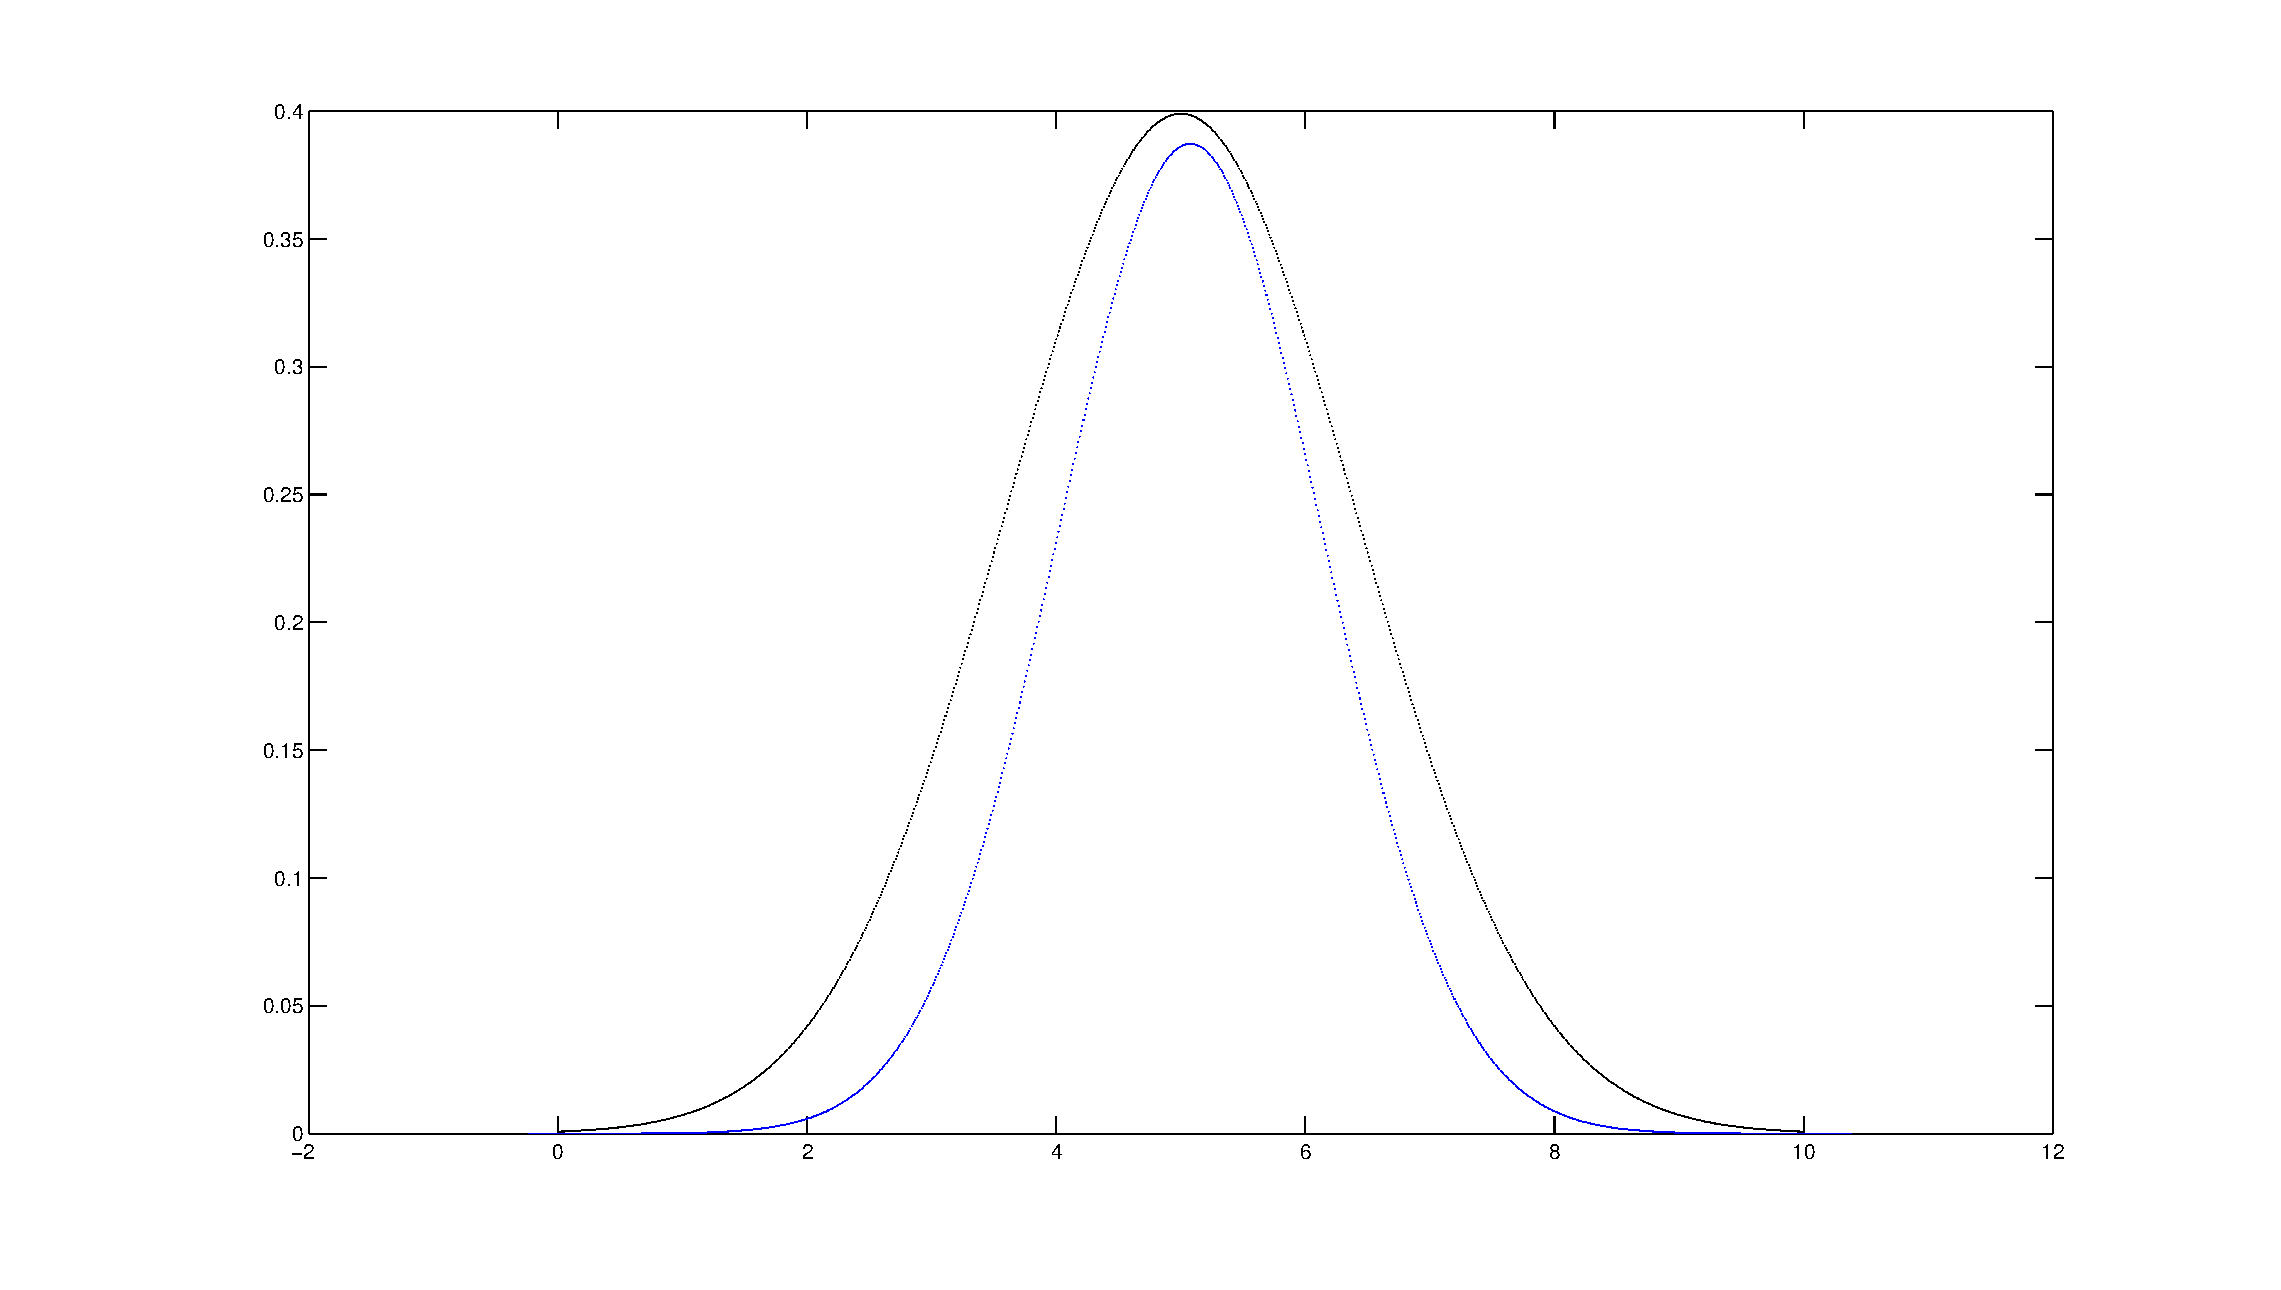
\includegraphics[scale=0.4]{gauss-gauss}
\caption{}
\end{figure}

\begin{figure}
\label{}
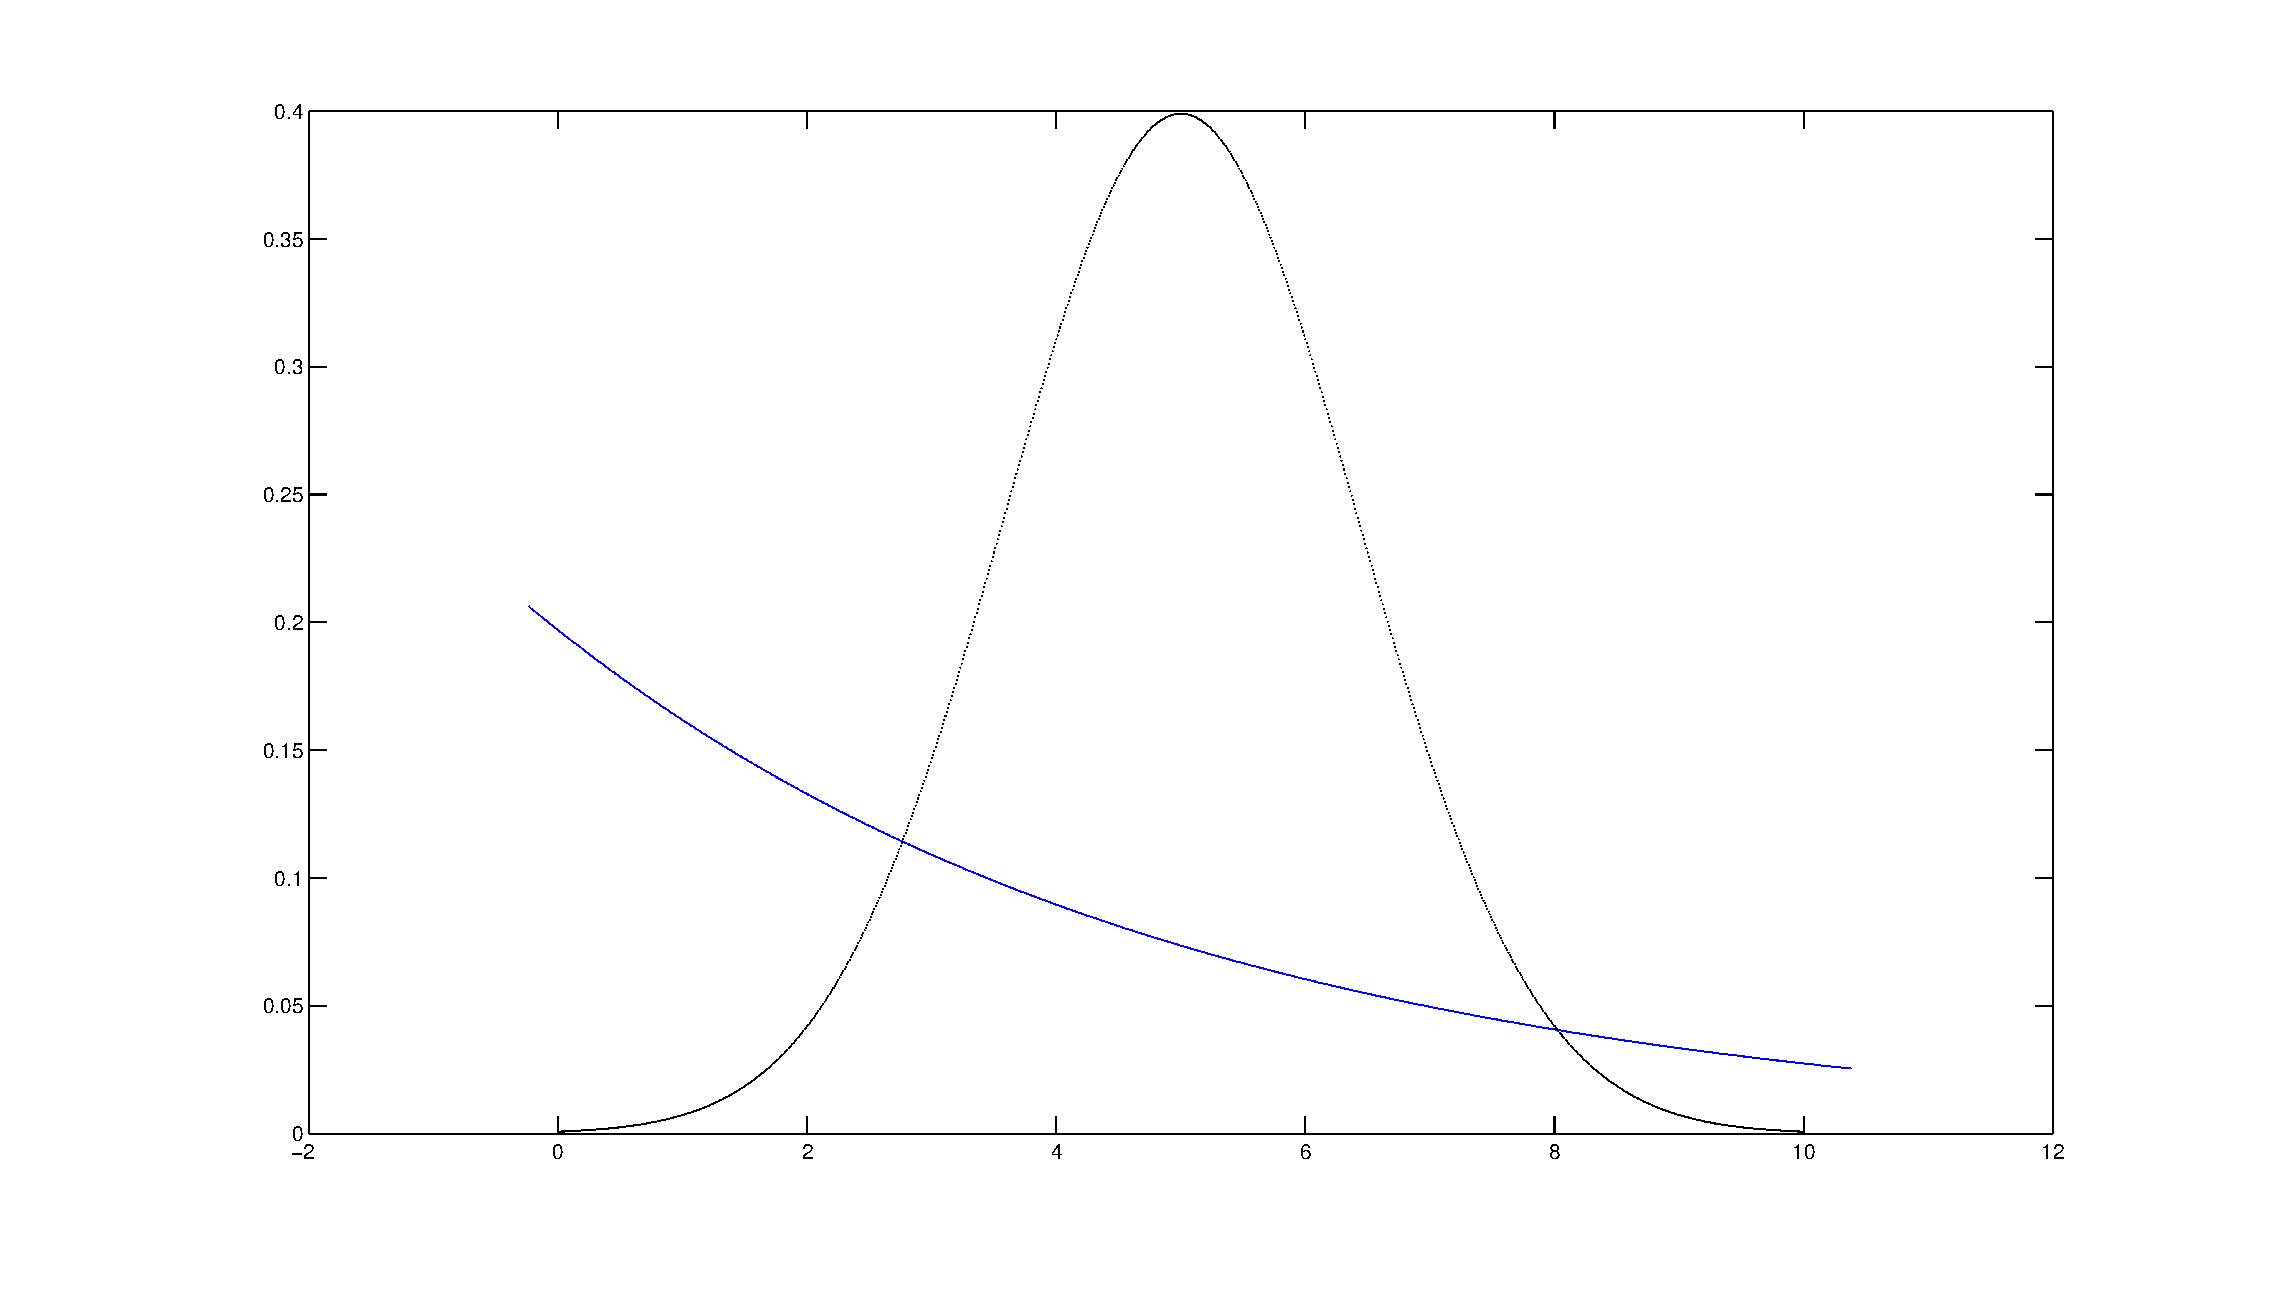
\includegraphics[scale=0.4]{gauss-exp}
\caption{}
\end{figure}

\begin{figure}
\label{}
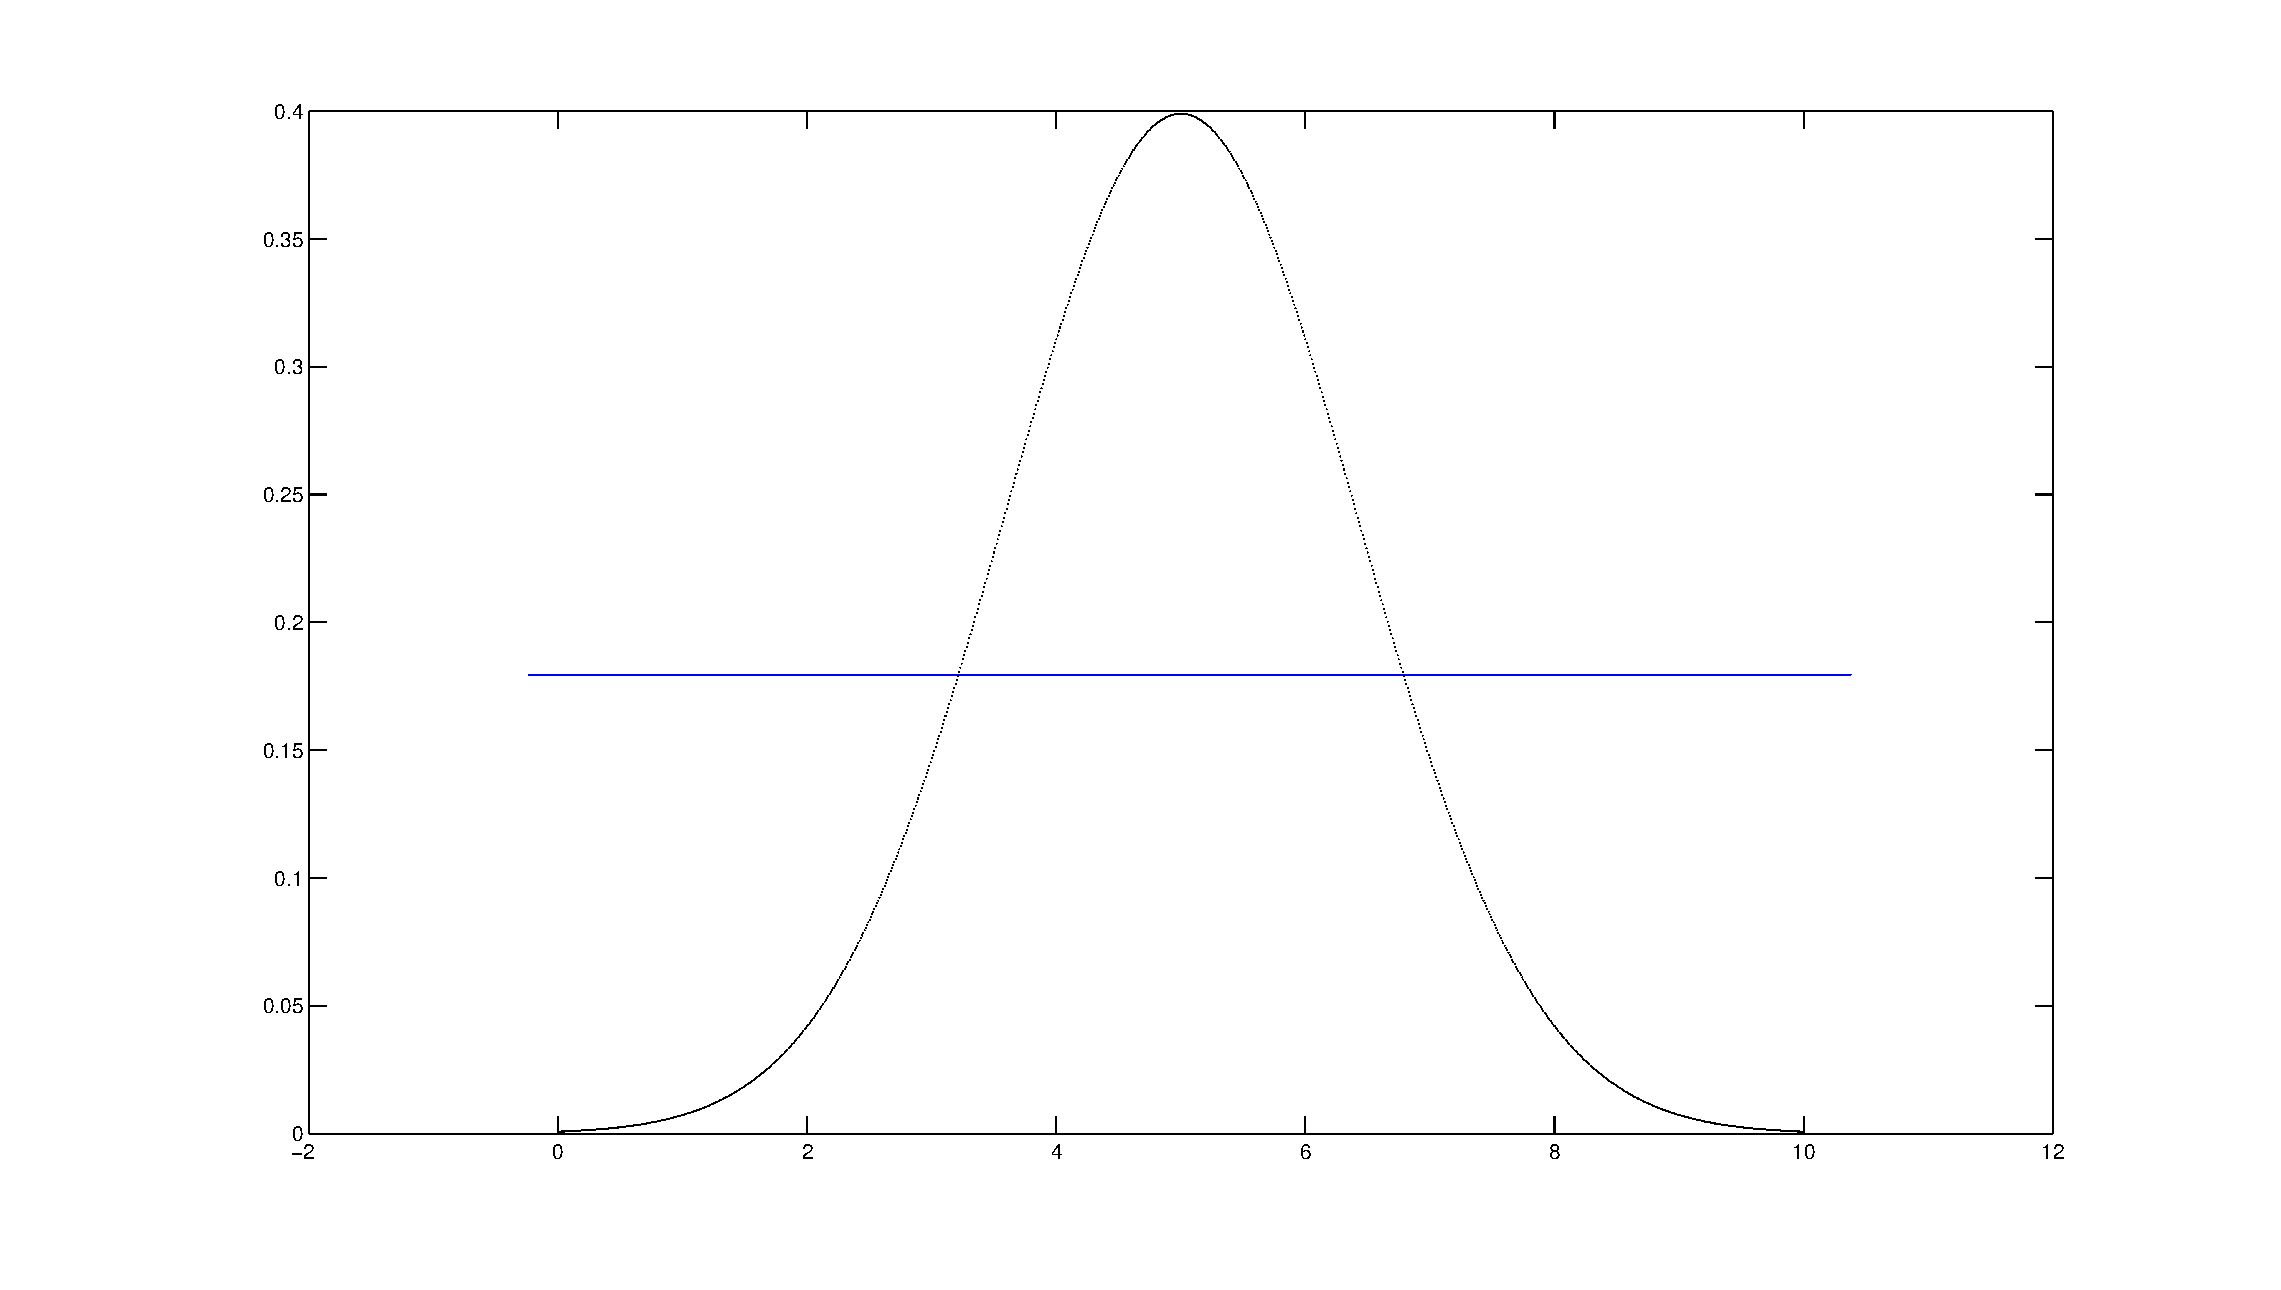
\includegraphics[scale=0.4]{gauss-uni}
\caption{}
\end{figure}

\begin{figure}
\label{}
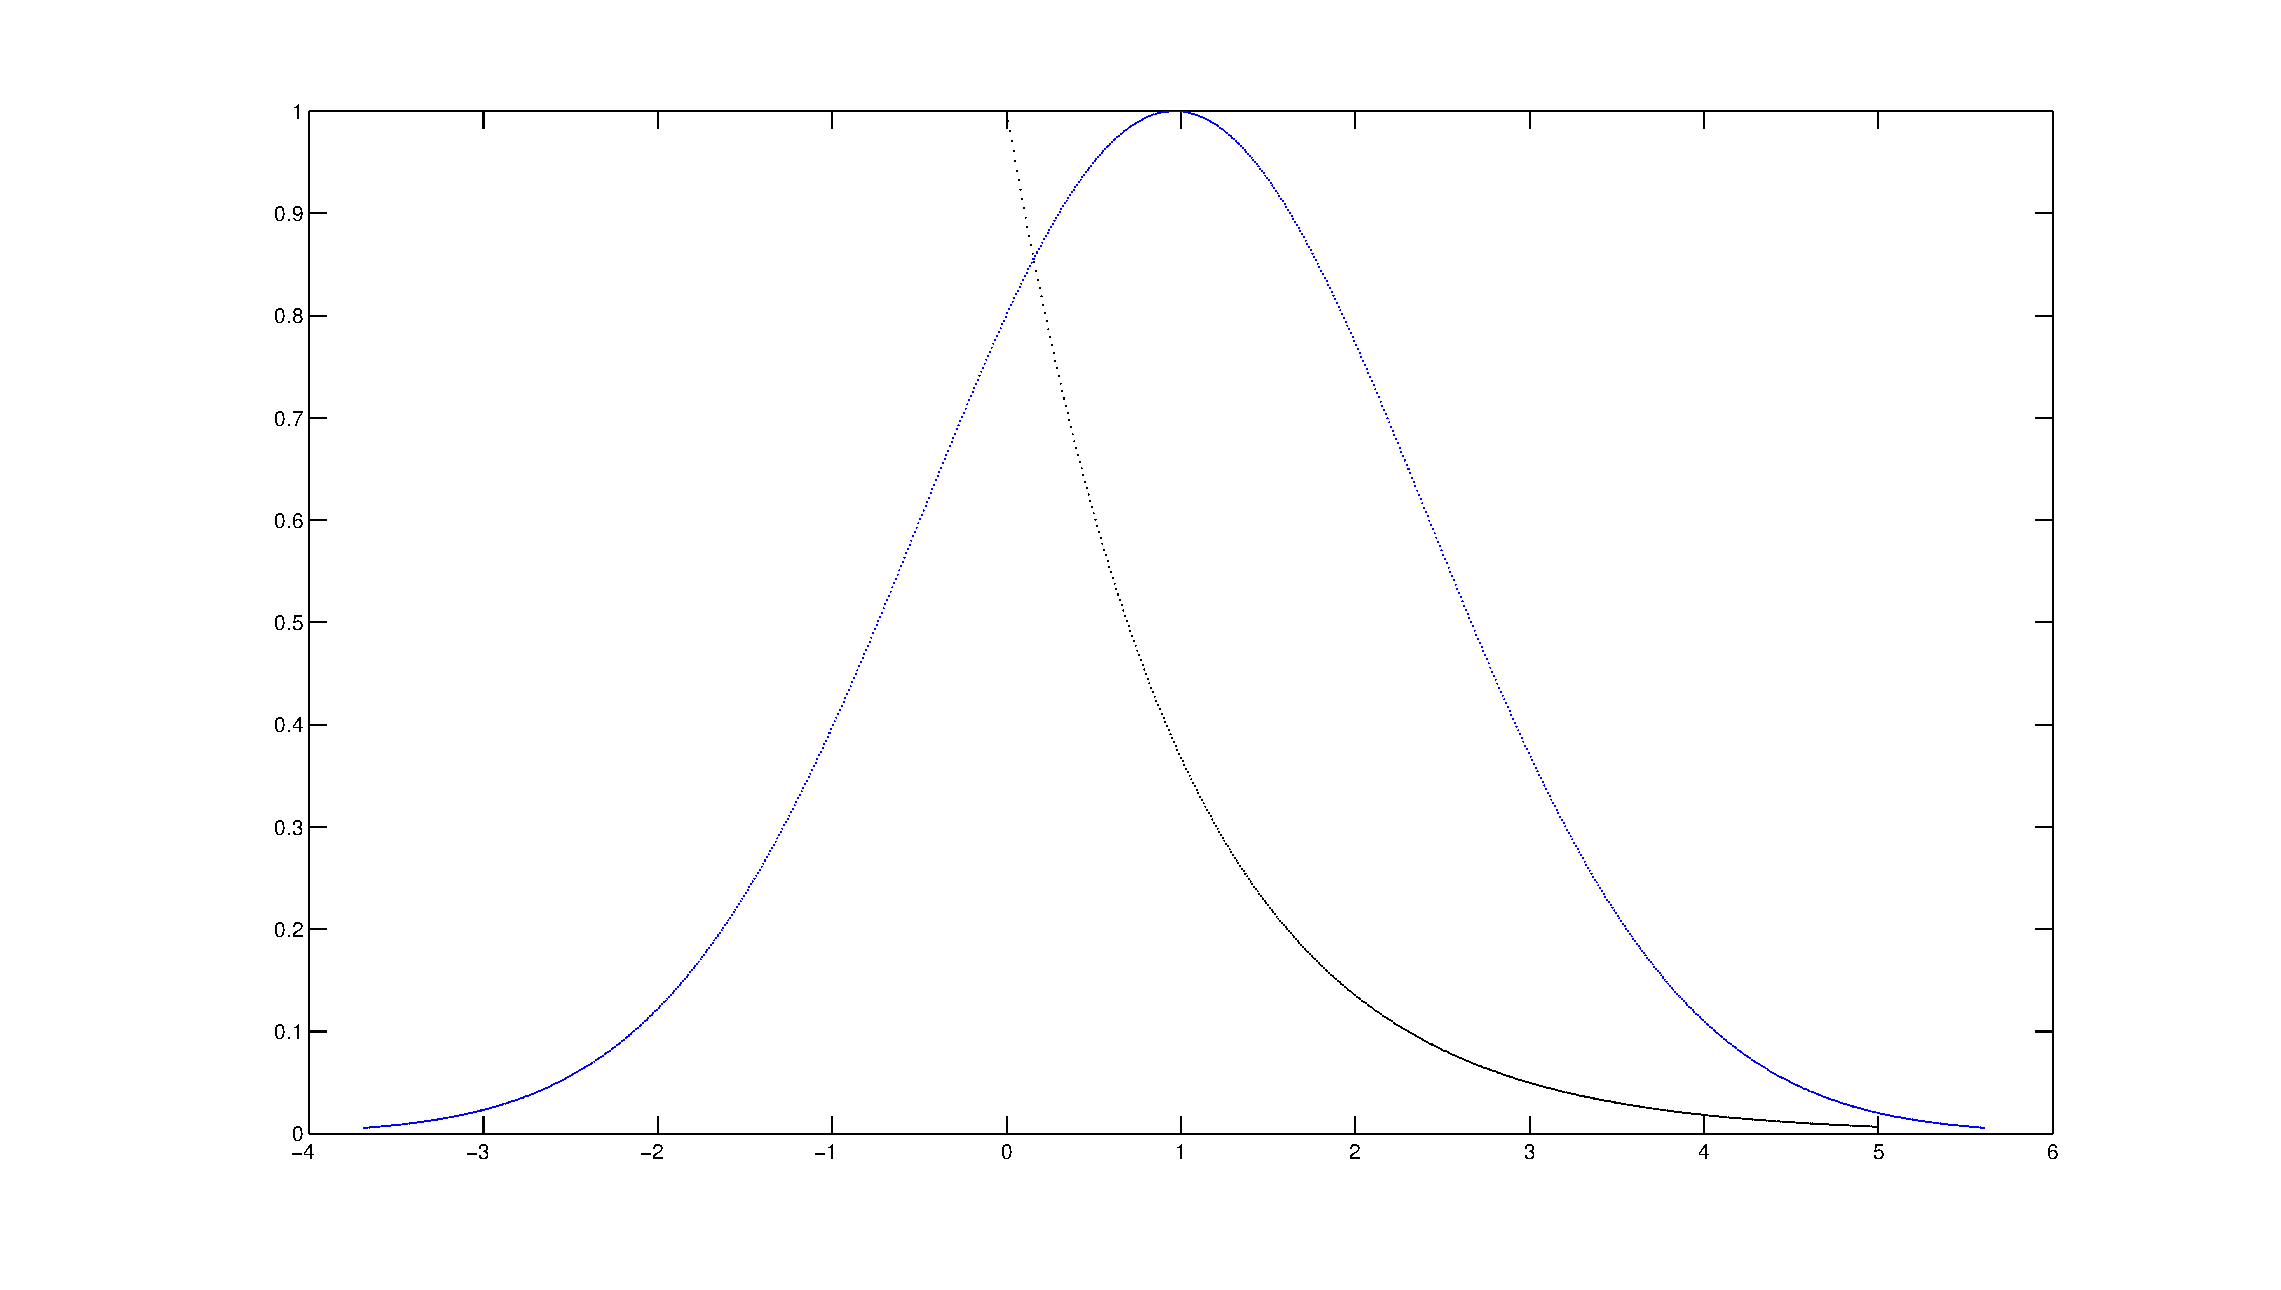
\includegraphics[scale=0.4]{exp-gauss}
\caption{}
\end{figure}

\begin{figure}
\label{}
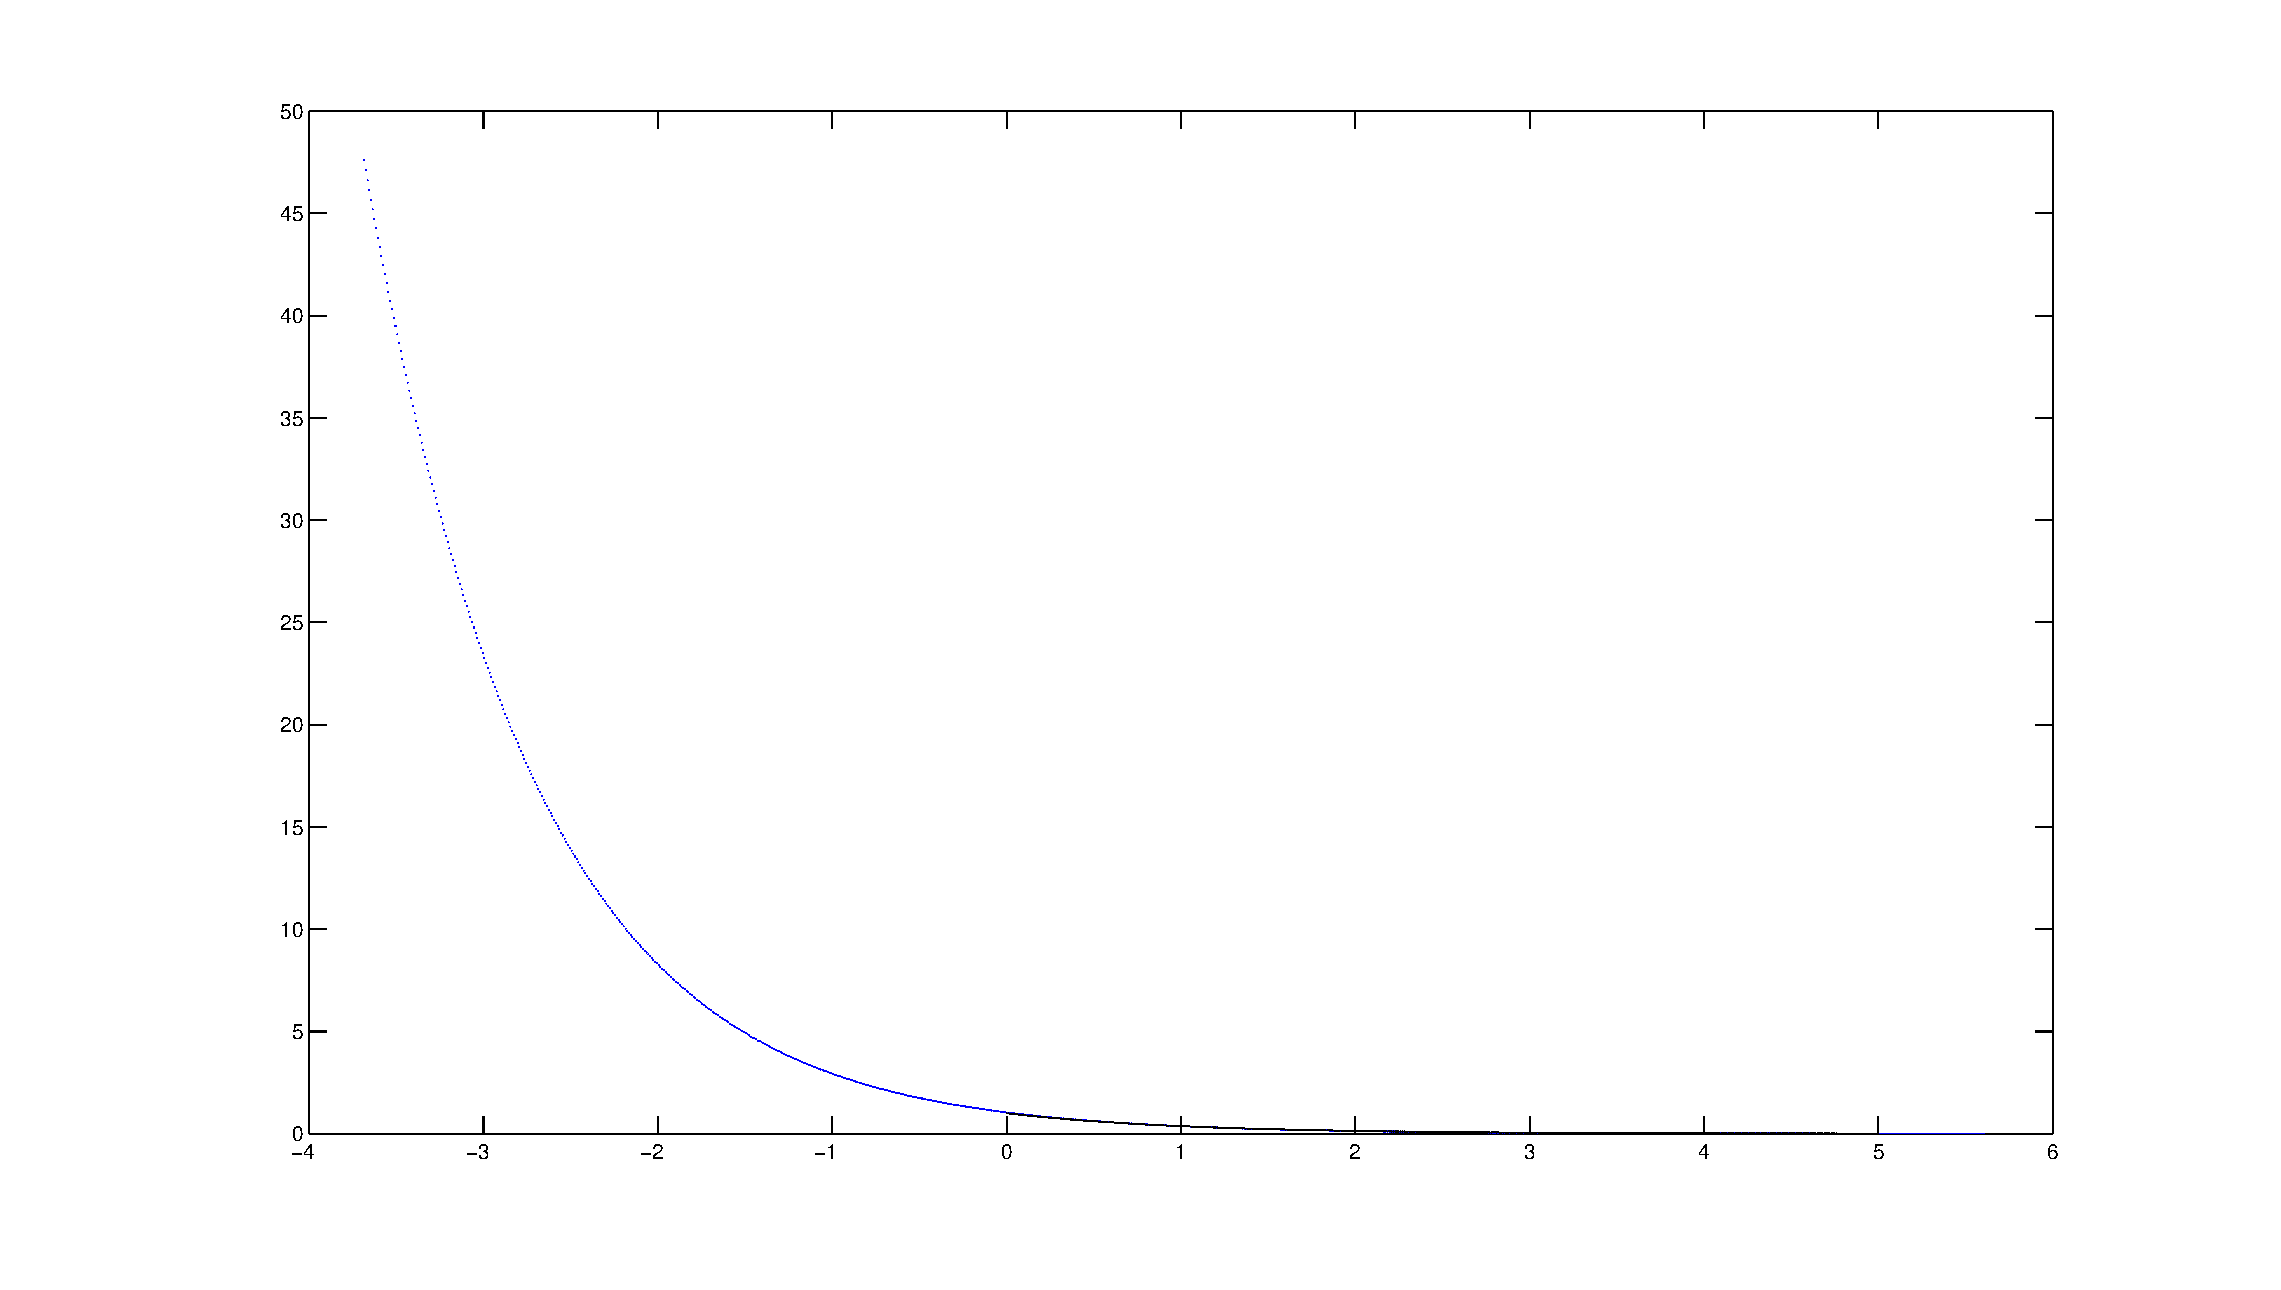
\includegraphics[scale=0.4]{exp-exp}
\caption{}
\end{figure}

\begin{figure}
\label{}
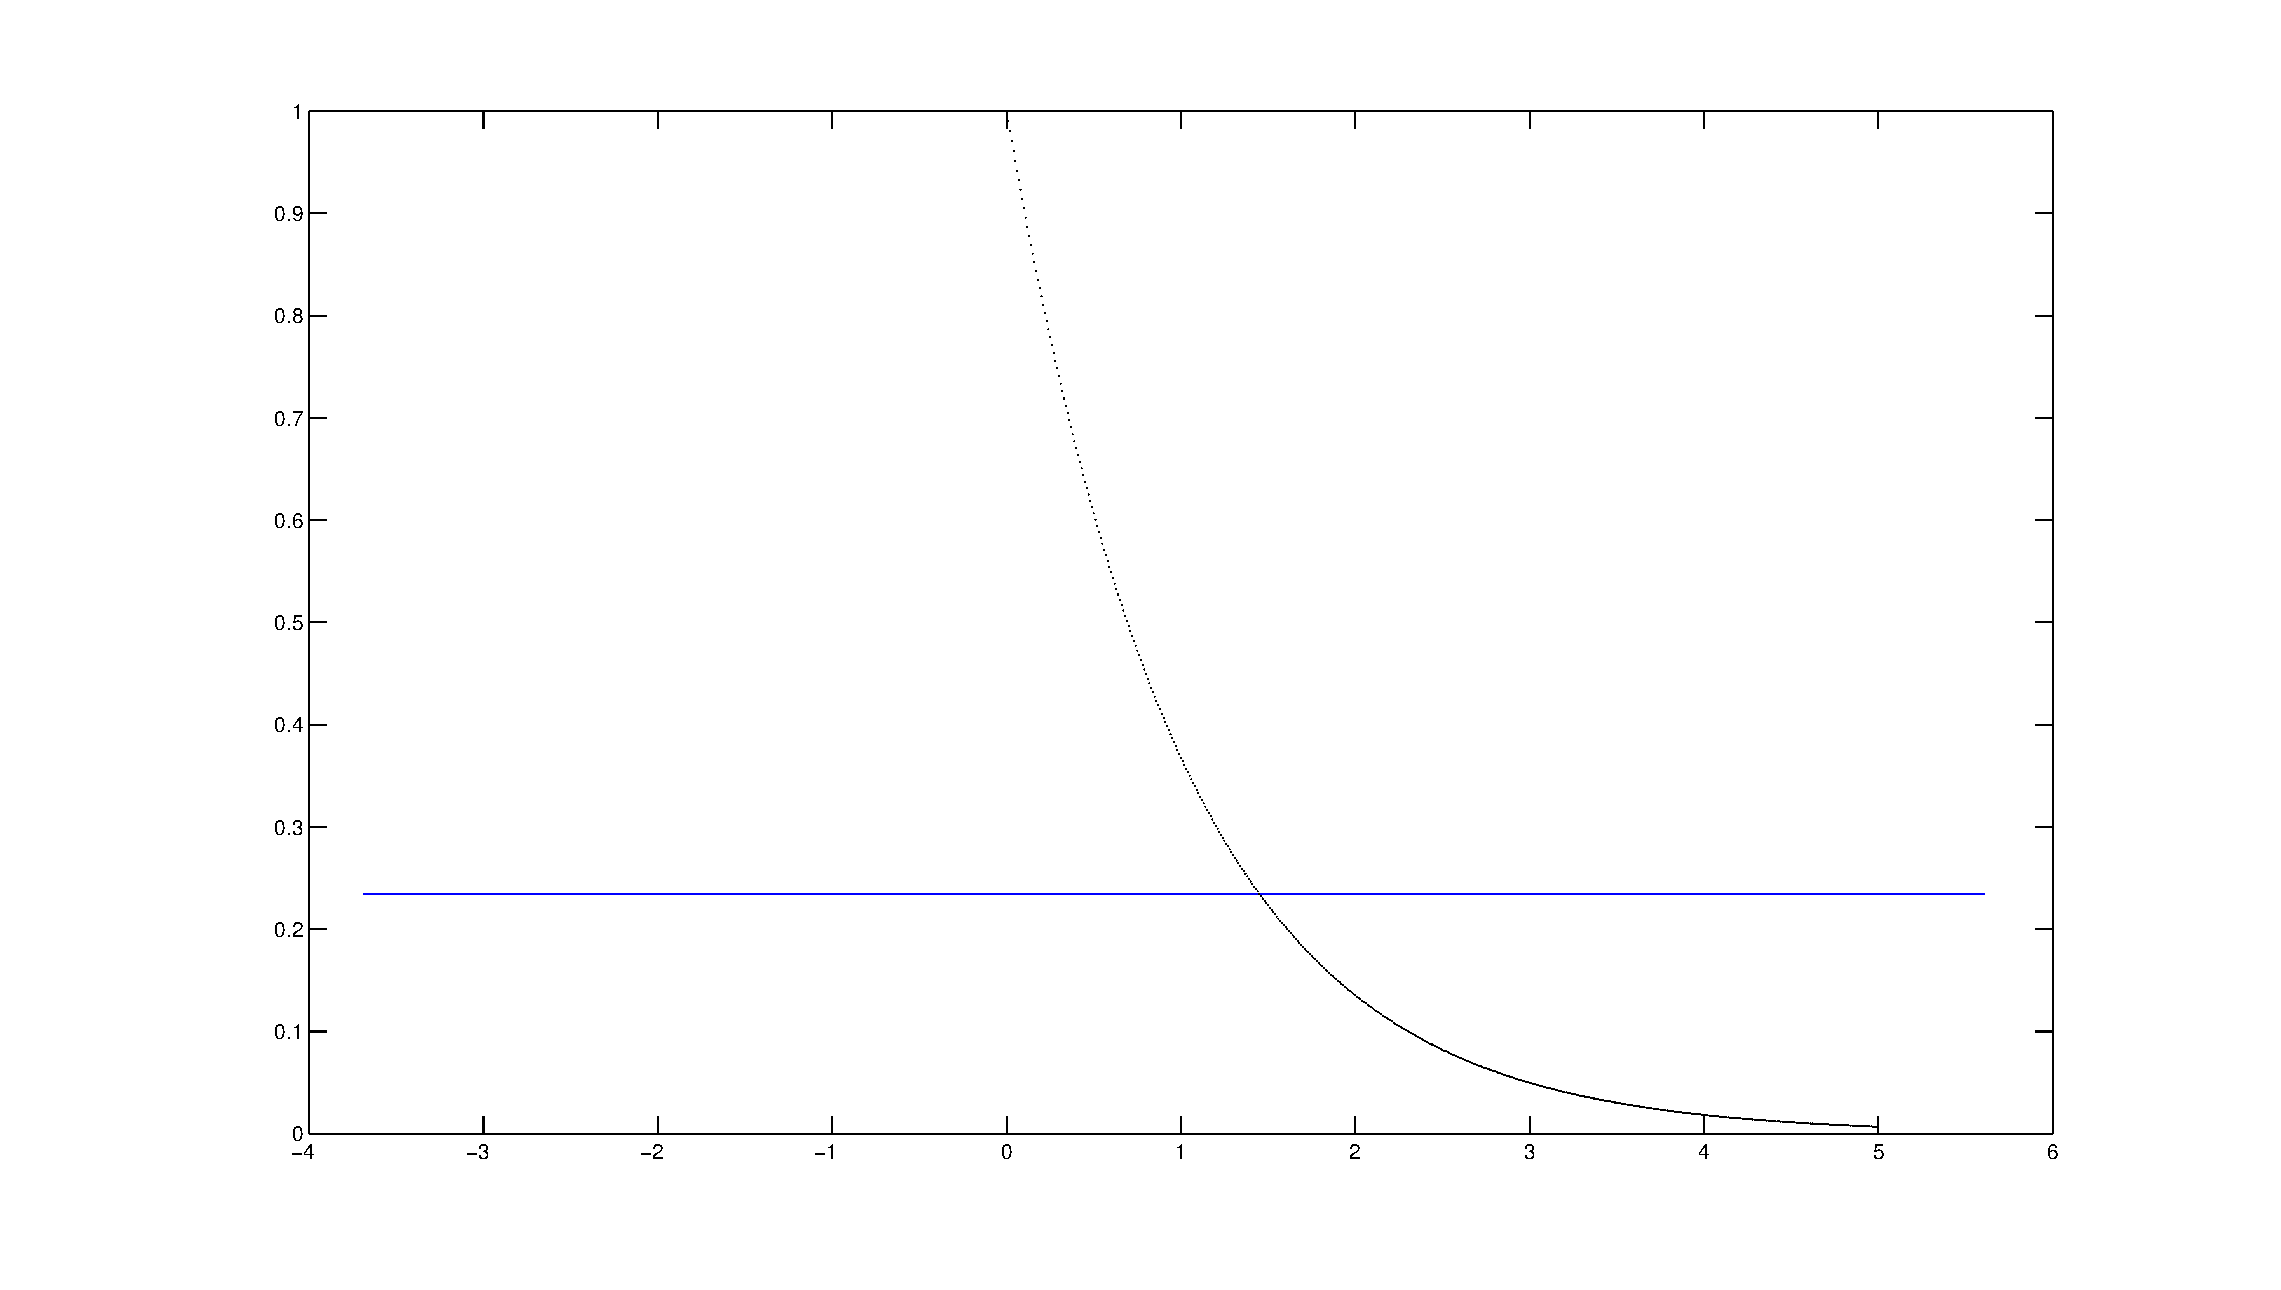
\includegraphics[scale=0.4]{exp-uni}
\caption{}
\end{figure}

\begin{figure}
\label{}
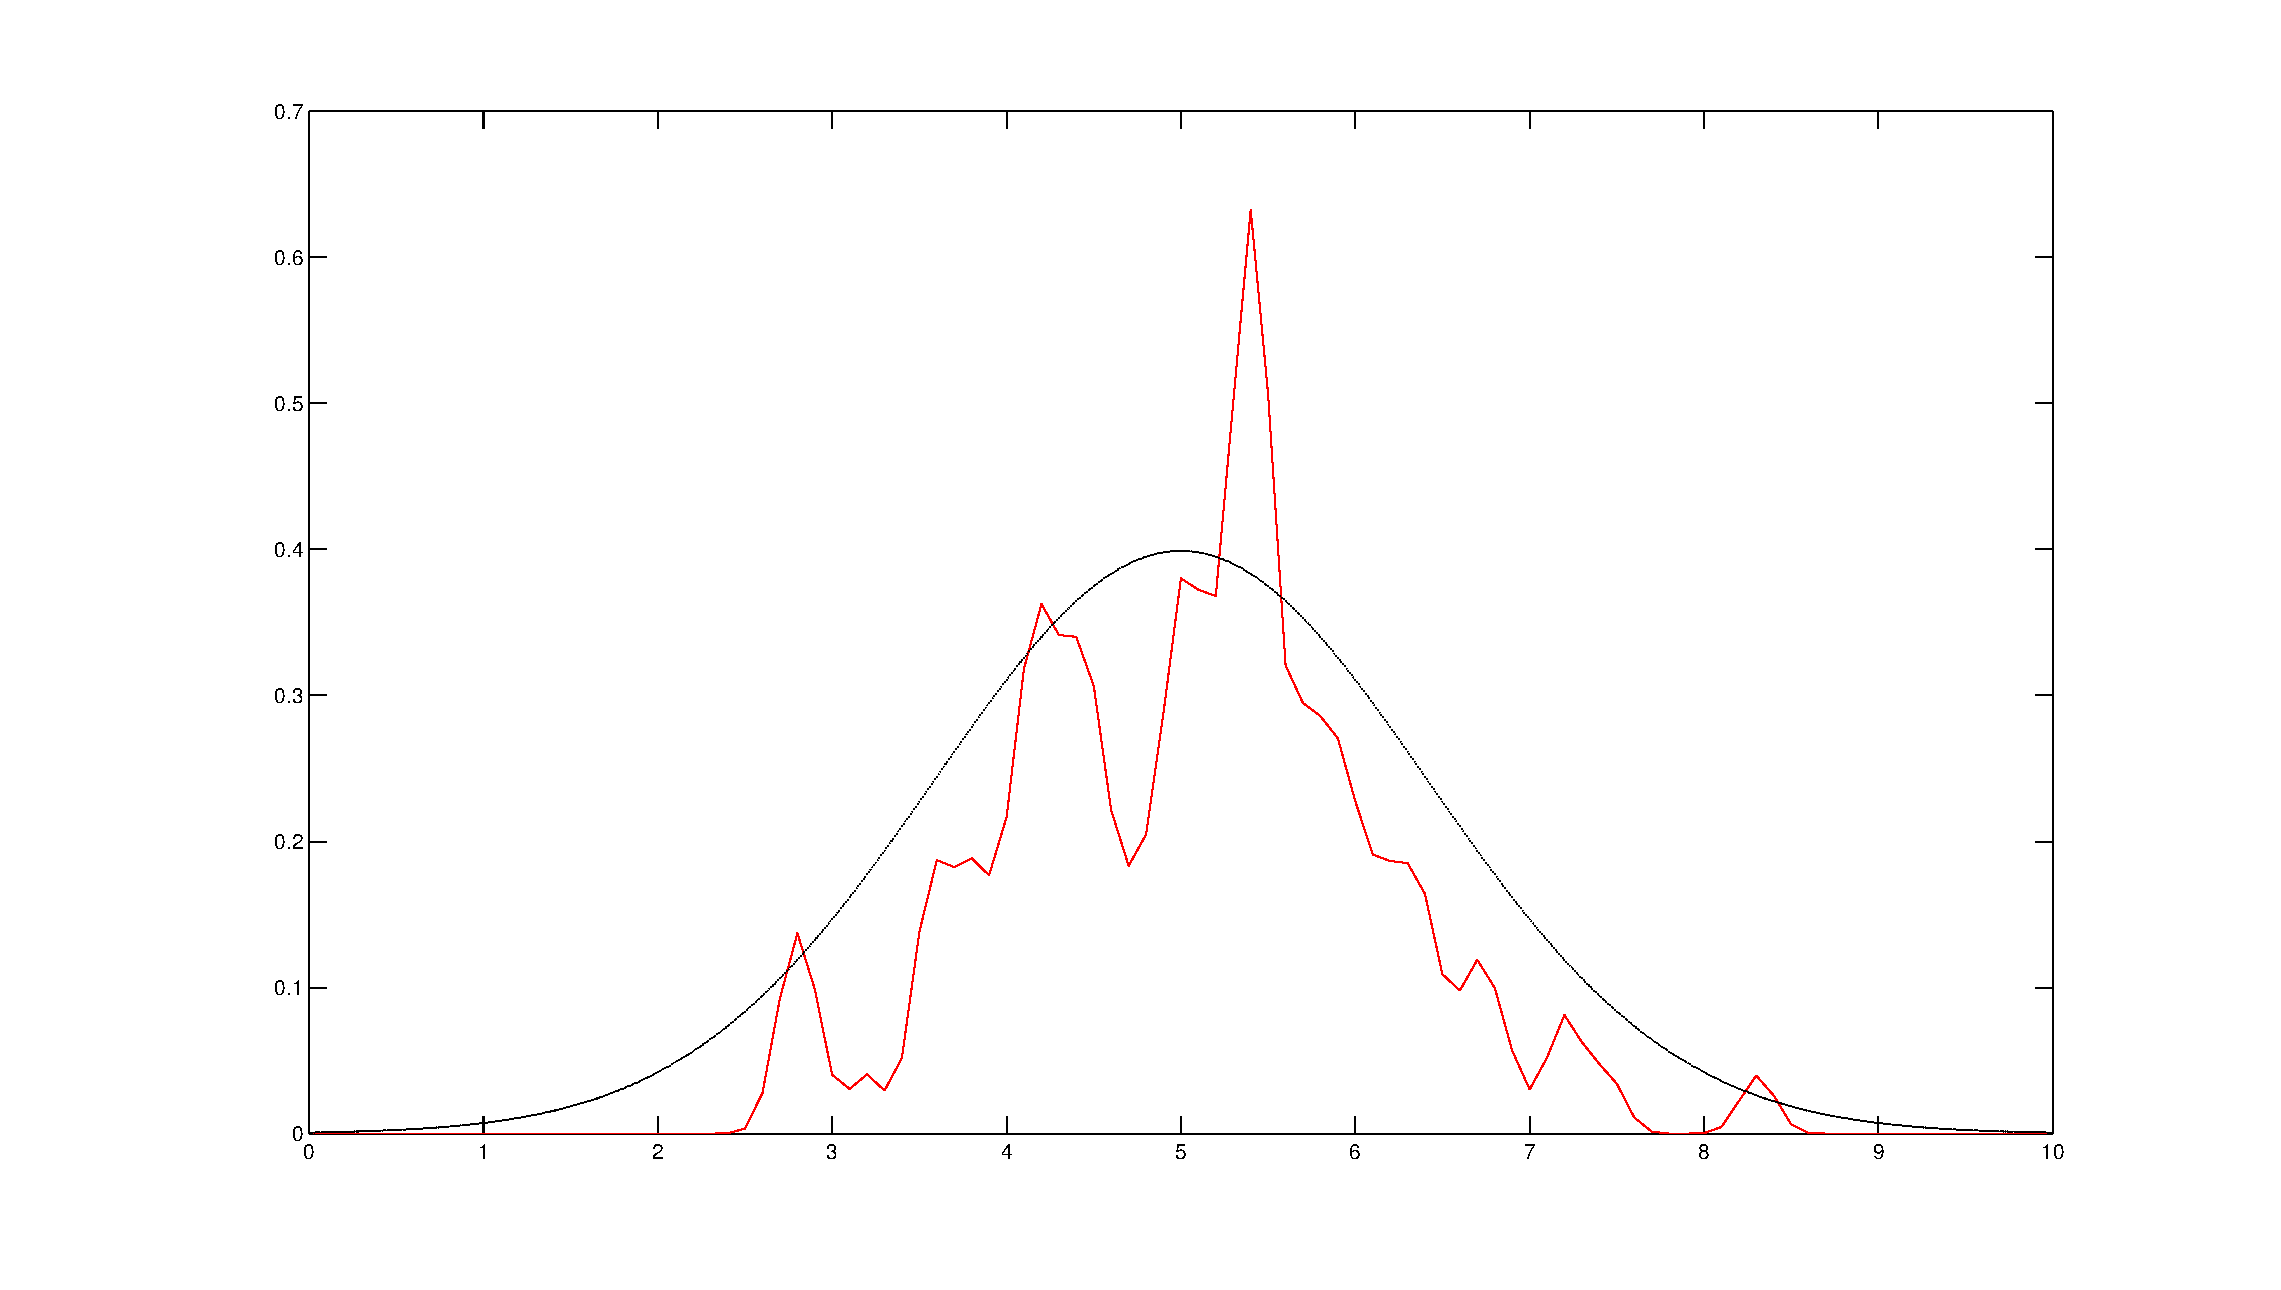
\includegraphics[scale=0.4]{nonpar-parzen-01}
\caption{}
\end{figure}

\begin{figure}
\label{}
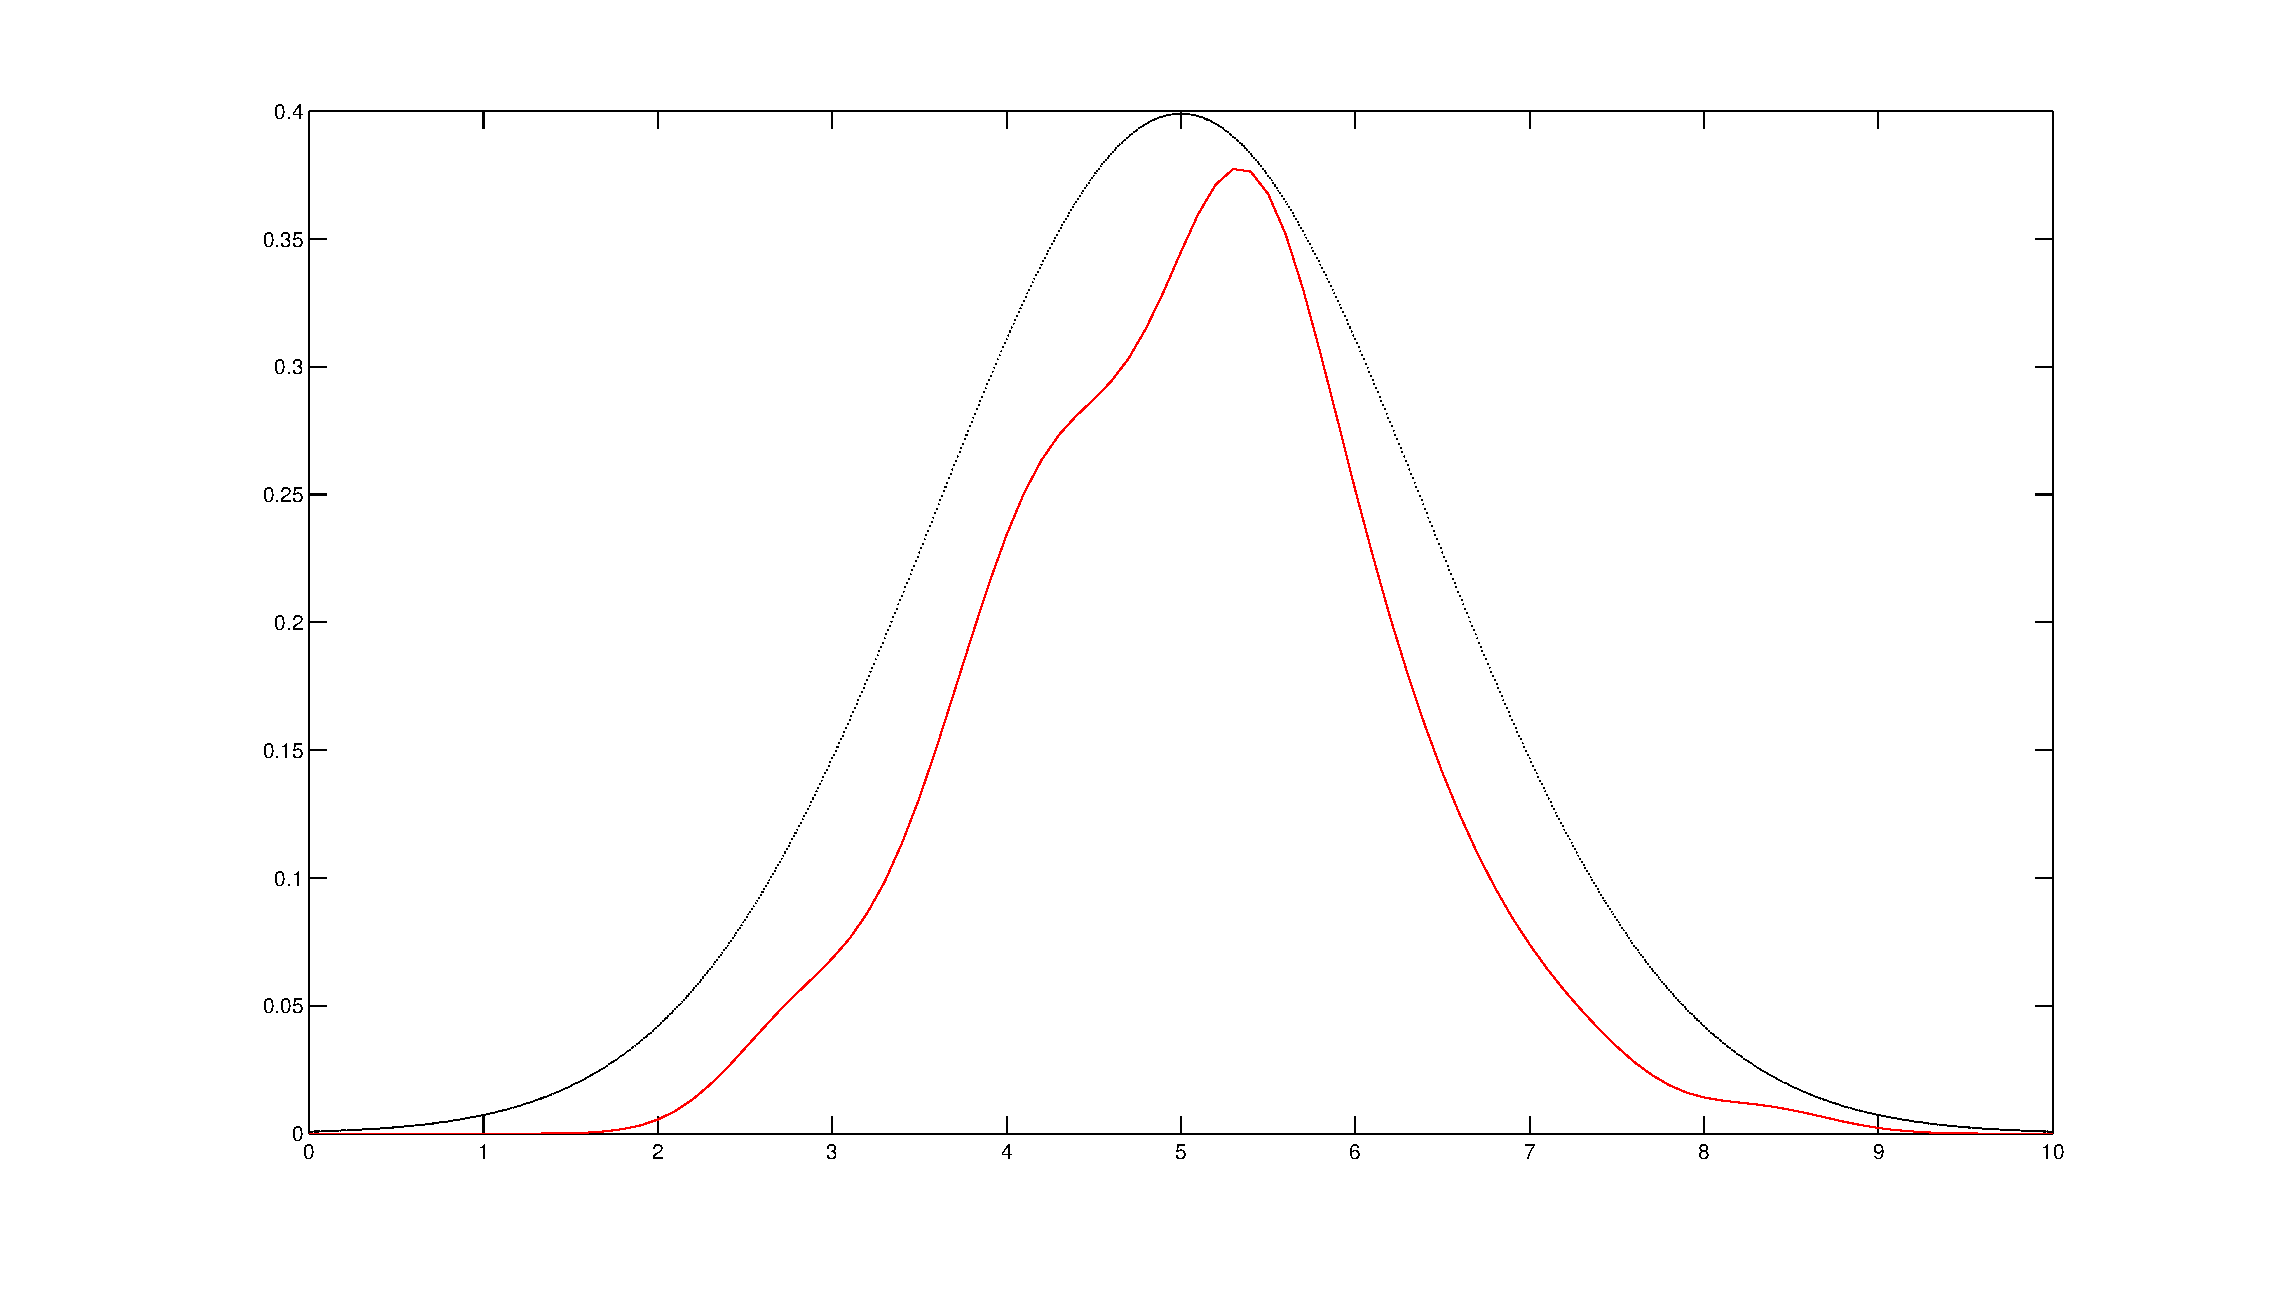
\includegraphics[scale=0.4]{nonpar-parzen-04}
\caption{}
\end{figure}